\documentclass{amsart}[12pt]
\usepackage{amsmath, amsfonts, tikz, natbib, array}
\usetikzlibrary{patterns}
\oddsidemargin=0in \evensidemargin=0in
\textwidth=6.6in \textheight=8.7in

\title{Map projections between Euclidean and spherical quadrilaterals}
\author{B R S Recht}
\date{April 2020}

\begin{document}
\maketitle
\tableofcontents

\section{Introduction}
A small but persistent trend in creating world maps has been to map onto a
polyhedron, and then unfold the polyhedron into a flat polyhedral net.
Most maps in this category use regular polyhedra, often the cube or the
icosahedron (in Fuller's second Dymaxion map).\cite{gray94} Other polyhedra include the other regular solids and
some Archimedean solids; Fuller used the cuboctahedron for his first Dymaxion
map,\cite{gray95} and the truncated icosahedron was used by
Snyder.\cite{snyder92} Maps between a polygon and a hemisphere
can be considered as polyhedral maps if the dihedron is
allowed.\cite{snyder89}\cite{lambers} The inverse mapping can be used to
inscribe a grid on a sphere, as in the quadrilateralized spherical
cube\cite{chan75}\cite{oneill76} or discrete global grids.\cite{sahr98}

Another is
the field of computer graphics, where there is some interest in functions
between the square to the disk.\cite{fong15}\cite{fong18}
These functions can be composed with an appropriate map
projection from the disk to the hemisphere
to create a map projection between the square and the sphere.\cite{lambers}

Nearly all of the literature on map projections between Euclidean and spherical
polygons, either in general or particular, only deals with regular polygons.
However, geographical features do not follow any regular geometric rules.
Regular polygons are mathematically easier to study, but irregular polygons are
also tractable. In this text, map projections between general Euclidean and
spherical polygons will be described. Some of these are extensions of existing
map projections, while some are new compromise map projections.

\section{Preliminaries}
Let $(u,v)$ be a vector in $\mathbb R^2$, and $\zeta = u + i v$ be the
corresponding complex number in $\mathbb C$ or the Riemann sphere $\mathbb C
\cup \{\infty\}$. Which notation is used will depend on the mapping:
conformal maps are best expressed in terms of complex variables.

\subsection{Spherical geometry with 3-vectors}
Some of the map projections to be discussed are better expressed
in terms of a vector rather than latitude and longitude. This text will only
cover pertinent details: a fuller description can be found in e.g. \cite{gade}.

Let $\phi \in [-\frac{\pi}{2}, \frac{\pi}{2}]$ be latitude, and
$\lambda \in (-\pi, \pi]$ be longitude. Let $\mathbf v = (x, y, z)$ be a vector
in $\mathbb R^3$ and $\mathbf{\hat{v}} = (x, y, z)$ be a unit vector on the
sphere $S^2$ such that $\| \mathbf{\hat{v}} \| = \sqrt{x^2 + y^2 +z^2} = 1$.
To convert from latitude and longitude to a unit vector:
\begin{equation}
  \mathbf{\hat{v}} = \left(\sin (\phi), \sin (\lambda) \cos (\phi),
  -\cos (\lambda) \cos (\phi) \right)
\end{equation}
To convert from the unit vector $\mathbf{\hat{v}}$ to latitude and longitude:
\begin{equation}\begin{split}
  \phi &= \arcsin (x) = \arctan (x, \sqrt{y^2 + z^2}) \\
  \lambda &= \arctan (y, -z)
\end{split}\end{equation}

Often in this text we'll normalize a vector to make it a unit vector.
For brevity,
we'll notate this pre-normalized vector as $\mathbf{\widetilde{v}}$, such that
\begin{equation}
  \mathbf{\hat{v}} = \frac{\mathbf{\widetilde{v}}}{\|\mathbf{\widetilde{v}}\|}
\end{equation}

\subsubsection{Great circles}
The shortest distance (geodesic) between two points in Euclidean space is a
straight line. On the sphere, the shortest distance is an arc of the great
circle between those points. That distance is the central angle $\theta$
between the two points. There are a few vector forms for it, the most
numerically stable one being the one using $\arctan$.
\begin{equation}\begin{split}
\theta &= \arccos \left(\mathbf{\hat{v}}_1 \cdot \mathbf{\hat{v}}_2\right) \\
&= \arcsin \left(\|\mathbf{\hat{v}}_1 \times \mathbf{\hat{v}}_2\| \right) \\
&= \arctan \left( \frac{\|\mathbf{\hat{v}}_1 \times \mathbf{\hat{v}}_2\|}
  {\mathbf{\hat{v}}_1 \cdot \mathbf{\hat{v}}_2} \right)
\end{split}\end{equation}

The great circle is the intersection of the sphere
and a plane passing through the origin. A plane through the origin can be
specified as $\hat{\mathbf n} \cdot \mathbf v = 0$, where $\hat{\mathbf n}$ is
a unit vector normal to the plane; this vector $\hat{\mathbf n}$ can be used to
specify a great circle. Given two points $\mathbf{\hat{v}_1, \hat{v}_2}$ on the
sphere, the $\hat{\mathbf n}$ of the great circle between those two points is
(up to normalization) their cross product:
\begin{equation}
  \mathbf{\widetilde{n}} = \mathbf{\hat{v}}_1 \times \mathbf{\hat{v}}_2
\end{equation}
Two great circles intersect at two antipodal points on the sphere. The points
of intersection can be found as the cross product of the great circle normals:
\begin{equation}
  \mathbf{\widetilde{v}} = \pm \mathbf{\hat{n}}_1 \times \mathbf{\hat{n}}_2
\end{equation}

\subsubsection{Interpolation}
Interpolation in Euclidean space is standard linear interpolation. On the
sphere, interpolation is given by spherical linear interpolation, or slerp.
\begin{equation}
\mathrm{Lerp}(\mathbf{v_1}, \mathbf{v_2}; t) =
       (1-t) \mathbf{v_1} + t \mathbf{v_2}
\end{equation}
\begin{equation}
\mathrm{Slerp}(\mathbf{\hat{v}_1}, \mathbf{\hat{v}_2}; t) =
        \frac{\sin ((1-t)w)}{\sin (w)} \mathbf{\hat{v}_1} +
       \frac{\sin (tw)}{\sin (w)} \mathbf{\hat{v}_2}
\end{equation}
where $w = \arccos \mathbf{\hat{v}_1} \cdot \mathbf{\hat{v}_2}$. If $\mathbf{\hat{v}_1} = \mathbf{\hat{v}_2}$, then define $\mathrm{Slerp}(\mathbf{\hat{v}_1}, \mathbf{\hat{v}_2}; t) =
\mathbf{\hat{v}_1} = \mathbf{\hat{v}_2}$ for all $t$.

\subsubsection{Face normal}
For the purposes of this text, we define the normal to a (Euclidean) polygon as
so, where $n$ is the number of vertices in the polygon and
$i = 0 \dots n-1$ is an index for each vertex:
\begin{equation}
  \mathbf{\widetilde{n}} =
  \sum^{n-1}_i \mathbf{v}_i \times \mathbf{v}_{i+1}
\end{equation}
$i$ should be treated as if it's mod $n$, so that it loops around.
This definition allows for a somewhat sensible extension to skew polygons:
the normal points in a generally reasonable direction when applied to a skew
polygon. The normal will be outward-facing if the points are ordered
counterclockwise, and inward-facing if the points are ordered clockwise.

\subsection{Euclidean spaces and transformations, including $uv$ coordinates}
This text uses barycentric coordinates on Euclidean triangles.
Quadrilaterals are instead specified by \textit{$uv$ coordinates} where
$u$ and $v$ are $\in [-1, 1]$. The subset of the plane $[-1, 1]^2$ is termed
the standard square. Here we discuss transformations of those

\subsubsection{Affine transformation}
Affine transformations are combinations of reflection, scaling, rotation,
shearing, and translation. This can be expressed as $\mathbf v = \mathbf A [u,
v]^T + v_0$, where $\mathbf A$ is a matrix. However, it is often more
convenient to express affine transformations using an augmented matrix like so:
\begin{equation}
  \begin{bmatrix}  x \\  y \\  1 \end{bmatrix}
   = \mathbf M
    \begin{bmatrix}  u \\  v \\  1 \end{bmatrix},\,
    \mathbf M = \begin{bmatrix}
       A_{11} & A_{12} & v_{0x} \\
       A_{21} & A_{22} & v_{0y} \\
       0 & 0 & 1
       \end{bmatrix}
\end{equation}
The transformation is invertible if $\mathbf M$ (or $\mathbf A$) is
invertible. This transformation can also transform between spaces of different
dimension, although then $\mathbf M$ is not a square matrix.

Affine transformations are equal-area in the sense defined earlier if
$|\mathbf M| \ne 0$, so if using an equal-area projection it may be desirable
to limit oneself to affine transformations. If $|\mathbf M| = 1$, then it defines a conformal affine transformation, effectively a combination of translation and rotation.

\subsubsection{Homography}
Homography, or projective transformation, is commonly used in computer vision
and graphics to handle objects seen in perspective, and may be convenient in
some software environments. A homography may be given by:
\begin{equation}
  \begin{bmatrix} xt \\ yt \\ t \end{bmatrix}
  = \mathbf{M} \begin{bmatrix} u  \\ v \\ 1  \end{bmatrix}
\end{equation}
where $\mathbf{M}$ is called the matrix of the homography. The matrix is
defined up to multiplication by a positive constant: $\mathbf{M}$ and
$k\mathbf{M}$ where $k>0$ define the same homography. The inverse of this
transformation is also a projective transformation, with matrix of the
homography $\mathbf{M}^{-1}$. Given 4 points in the $uv$ plane and their target
in the $xy$ plane, $\mathbf{M}$ can be determined as the null-space of this
system:
\begin{equation}
  \begin{bmatrix}
  x_1 & x_1 u_1 & x_1 v_1 & -1 & -u_1 & -v_1 & 0 & 0 & 0 \\
  x_2 & x_2 u_2 & x_2 v_2 & -1 & -u_2 & -v_2 & 0 & 0 & 0 \\
  x_3 & x_3 u_3 & x_3 v_3 & -1 & -u_3 & -v_3 & 0 & 0 & 0 \\
  x_4 & x_4 u_4 & x_4 v_4 & -1 & -u_4 & -v_4 & 0 & 0 & 0 \\
  y_1 & y_1 u_1 & y_1 v_1 & 0 & 0 & 0 & -1 & -u_1 & -v_1 \\
  y_2 & y_2 u_2 & y_2 v_2 & 0 & 0 & 0 & -1 & -u_2 & -v_2 \\
  y_3 & y_3 u_3 & y_3 v_3 & 0 & 0 & 0 & -1 & -u_3 & -v_3 \\
  y_4 & y_4 u_4 & y_4 v_4 & 0 & 0 & 0 & -1 & -u_4 & -v_4
   \end{bmatrix}
   \begin{bmatrix}
  M_{11} \\ M_{12} \\ M_{13} \\
  M_{21} \\ M_{22} \\ M_{23} \\
  M_{31} \\ M_{32} \\ M_{33}
  \end{bmatrix} = \mathbf{0},
\end{equation}
where
\begin{equation}
  \mathbf{M} = \begin{bmatrix}
  M_{11} & M_{12} & M_{13} \\
  M_{21} & M_{22} & M_{23} \\
  M_{31} & M_{32} & M_{33} \end{bmatrix}.
\end{equation}
This transformation can also be adapted to a transform from 2-d $uv$ space to a
plane in 3-d $xyz$ space. The target points must be coplanar, and since the
matrix of the homography is now a 3 by 4 matrix, the inverse transformation is
given by the pseudoinverse instead. Homographies are undefined along the line
where $t=0$, but this rarely becomes an issue in the context of this text.

\subsubsection{Bilinear Interpolation}
\begin{figure}%[!htbp]
\begin{tikzpicture}
  \draw (0, 0) -- (4, 0) -- (4, 3) -- (1, 4) -- (0, 0);
  \draw[fill] (0, 0) circle [radius=0.05] node[anchor=east] {\tiny 1};
  \draw[fill] (4, 0) circle [radius=0.05] node[anchor=west] {\tiny 2};
  \draw[fill] (4, 3) circle [radius=0.05] node[anchor=west] {\tiny 3};
  \draw[fill] (1, 4) circle [radius=0.05] node[anchor=east] {\tiny 4};
  \draw[dotted] (2, 0) node[anchor=north] {\tiny 1,2}
    -- (2.5, 3.5) node[anchor=south] {\tiny 4,3};
  \draw[dotted] (0.5, 2) node[anchor=east] {\tiny 1,4}
    -- (4, 1.5) node[anchor=west] {\tiny 2,3};
  \draw[fill] (2.25, 1.75) circle [radius=0.05];
\end{tikzpicture}
\caption{Bilinear interpolation, showing intersection of lines.}
\label{fig:uv}
\end{figure}
Another transformation is usually called 'bilinear interpolation' in image processing applications. Let $\mathbf v_1, \mathbf v_2, \mathbf v_3, \mathbf v_4$ be points in 2-d or 3-d (or higher) space. Define:
\begin{equation}\begin{split}
\mathbf v_{1,2} & = \mathrm{Lerp}(\mathbf v_1,\mathbf v_2;\frac{u+1}{2}),\\
\mathbf v_{4,3} & = \mathrm{Lerp}(\mathbf v_4,\mathbf v_3;\frac{u+1}{2}),\\
\mathbf v_{1,4} & = \mathrm{Lerp}(\mathbf v_1,\mathbf v_4;\frac{v+1}{2}),\\
\mathbf v_{2,3} & = \mathrm{Lerp}(\mathbf v_2,\mathbf v_3;\frac{v+1}{2})
\end{split}\end{equation}
Then bilinear interpolation determines the point $\mathbf v$ as:
\begin{equation}\begin{split}
\mathbf v
& = \mathrm{Lerp}(\mathbf v_{1,2}, \mathbf v_{4,3}; \frac{v+1}{2}) \\
& = \mathrm{Lerp}(\mathbf v_{1,4}, \mathbf v_{2,3}; \frac{u+1}{2}) \\
& = \frac{(1-u)(1-v)}{4} \mathbf v_1 +
\frac{(1+u)(1-v)}{4} \mathbf v_2 +
\frac{(1+u)(1+v)}{4} \mathbf v_3 +
\frac{(1-u)(1+v)}{4} \mathbf v_4 \\
&= \mathbf{a} + u \mathbf{b} + v \mathbf{c} + u v \mathbf{d}
\end{split}\end{equation}
where
\begin{equation}\begin{split}
  \mathbf{a} &= \frac{\mathbf v_1 +\mathbf v_2 +\mathbf v_3 + \mathbf v_4}{4},
  \\
  \mathbf{b} &= \frac{-\mathbf v_1 +\mathbf v_2 +\mathbf v_3 - \mathbf v_4}{4},
  \\
  \mathbf{c} &= \frac{-\mathbf v_1 -\mathbf v_2 +\mathbf v_3 + \mathbf v_4}{4},
  \\
  \mathbf{d} &= \frac{\mathbf v_1 -\mathbf v_2 +\mathbf v_3 - \mathbf v_4}{4}
\end{split}\end{equation}
The $uv$ term in the transformation illustrates the choice of name: in 3d, if
the vertices $v_i$ are not coplanar, then the transformation maps the plane to
a hyperbolic paraboloid. Bilinear interpolation preserves evenly spaced points
along an edge of the quadrilateral defined by $v_i$, and avoids the undefined
space of the homography. However, the inverse function is somewhat more
complicated. The inverse of bilinear interpolation,
for $\mathbf{v}_i \in \mathbb{R}^2$, is given by:
\begin{equation}\begin{split}
 u &= \frac{-b_u + \sqrt{b_u^2 - 4 a_u c_u}}{2a_u}\\
 v &= \frac{-b_v + \sqrt{b_v^2 - 4 a_v c_v}}{2a_v}\\
 a_u &= \mathbf{b} \times \mathbf{d}, b_u = \mathbf{a} \times \mathbf{d} + \mathbf{b} \times \mathbf{c}, c_u = \mathbf{a} \times \mathbf{c},\\
 a_v &= \mathbf{c} \times \mathbf{d}, b_v = \mathbf{a} \times \mathbf{d} - \mathbf{b} \times \mathbf{c}, c_v = \mathbf{a} \times \mathbf{b},\\
\end{split}\end{equation}
where the 2d scalar cross product $\mathbf{a} \times \mathbf{b} = a_x b_y - b_x
a_y$ is used here. In more than two dimensions, pick two coordinates and use
those as $x$ and $y$.

If the shape is a planar parallelogram (or a special case of a parallelogram
like a rectangle), then $\mathbf v_1 + \mathbf v_3 = \mathbf v_2 + \mathbf v_4$,
and $\mathbf{d} = 0$. In this case, both the homography and the hyperbolic
paraboloid transformation reduce to an affine transformation. Qualitatively, homographies preserve all lines,
while bilinear interpolation preserves lines of constant $u$ or $v$.

Neither homographies nor bilinear interpolation are amenable to generalization
in the way that barycentric coordinates are. Bilinear interpolation can be
expressed like so:
\begin{equation}
  \mathbf v = \sum^4_{i=1} \alpha_i \mathbf v_i,
\end{equation}
but $\alpha_i$ are not necessarily unique for a given $\mathbf v$. Later we
will see some map projections that are similar in form to bilinear interpolation.

\subsection{Dealing with the ellipsoid}
The Earth is reasonably approximated as a sphere, and better approximated as a
slightly flattened oblate ellipsoid. In general this text will only deal with
the spherical approximation, but here we mention two considerations arising
from that approximation.

The vector form described in \cite{gade} corresponds to the geodetic latitude.
The mapping between the sphere and the ellipsoid using geodetic latitude is not
area-preserving, conformal, or distance-preserving, although the distortion is
small on the Earth ellipsoid. If applying an area-preserving, conformal, or
distance-preserving map projection, and the required precision is fine enough
that the distortion is a concern, the geodetic latitude can be substituted
with the authalic (equal-area), conformal, or rectifying
(equal-distance along meridians) latitude as described in \cite{snyder87}.
These can be calculated from the geodetic latitude,
and the difference is well-approximated by a Fourier series.

Considering polyhedral maps, in this text we require the edges of the polyhedra
to correspond to geodesics. Geodesics on a sphere are not necessarily geodesics
on an ellipse: as proof, geodesics on an ellipse are not necessarily closed,
while geodesics on a sphere are. (Of course, with the Earth ellipsoid, the
difference between the geodesics is small.) The equator and meridians are
geodesics on both surfaces, so if having exact geodesics is a concern,
place your polyhedron edges along the equator or meridians.

\section{Map projections}

\begin{figure}%[!htbp]
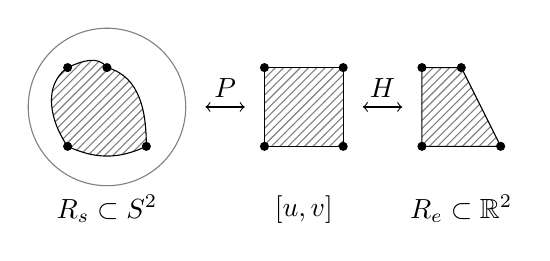
\begin{tikzpicture}
  \draw [gray] (9,1) circle [radius=1];
  \draw[pattern=north east lines, pattern color=gray] (8.5, 0.5) to [out=-25, in=205]
  (9.5, 0.5) to [out=90, in=-15]
  (9, 1.5) to [out=125, in=25]
  (8.5, 1.5) to [out=215, in=125]
  (8.5, 0.5);
  \draw[fill] (8.5,0.5) circle [radius=0.05];
  \draw[fill] (9.5,0.5) circle [radius=0.05];
  \draw[fill] (9,1.5) circle [radius=0.05];
  \draw[fill] (8.5,1.5) circle [radius=0.05];

  \draw [<->] (10.25,1) -- (10.75,1);
  \draw[pattern=north east lines, pattern color=gray] (11, 0.5) -- (12, 0.5) -- (12, 1.5) -- (11, 1.5) -- (11, 0.5);
  \draw[fill] (11,0.5) circle [radius=0.05];
  \draw[fill] (12,0.5) circle [radius=0.05];
  \draw[fill] (12,1.5) circle [radius=0.05];
  \draw[fill] (11,1.5) circle [radius=0.05];

  \draw [<->] (12.25,1) -- (12.75,1);
  \draw[pattern=north east lines, pattern color=gray] (13, 0.5) -- (14, 0.5) -- (13.5, 1.5) -- (13, 1.5) -- (13, 0.5);
  \draw[fill] (13,0.5) circle [radius=0.05];
  \draw[fill] (14,0.5) circle [radius=0.05];
  \draw[fill] (13.5,1.5) circle [radius=0.05];
  \draw[fill] (13,1.5) circle [radius=0.05];

\draw (10.5,1) node[anchor=south] {$P$};
\draw (12.5,1) node[anchor=south] {$H$};

\draw (9,0) node[anchor=north] {$R_s \subset S^2$};
\draw (11.5,0) node[anchor=north] {$[u,v]$};
\draw (13.5,0) node[anchor=north] {$R_e \subset \mathbb{R}^2$};

\end{tikzpicture}
\caption{Schematic for the application of most projections listed in this text.
Left: triangles, right: quadrilaterals. $P$ indicates the projection, $A$ is an affine transformation, and $H$ is a homography or bilinear interpolation.}
\label{fig:schematic}
\end{figure}

Figure \ref{fig:schematic} illustrates the general form of application of most
projections in this text. (Exceptions are noted in the relevant sections.) The
transformation from barycentric coordinates to the plane, or from $uv$
coordinates to a quadrilateral, takes the same form for each projection, so in
this section we can ignore that part except when there are special
considerations.

The polygon on the sphere $R_s$ and the polygon in the plane $R_e$ can be
basically anything, within the operating parameters of the projection and any
special considerations that may apply. Even with respect to each other, one
can be a regular polygon while the other is some irregular monster, if that is
desirable. Of course, this will influence the distortion of the map
projection.

The flip side of this freedom is that there is not
necessarily a unique way, given $R_s$, to choose $R_e$. If one is regular,
it may make sense to choose the other to also be regular. For irregular
triangles, one choice may be to choose $R_e$ such that its edges are
proportial in length to those of $R_s$. Another may be to choose $R_e$ to have
angles proportional to those of $R_s$: $\alpha' = \pi
\frac{\alpha}{\alpha+\beta+\gamma}$ etc. For quadrilaterals, it may be
desirable to carry over some quality from $R_s$ to $R_e$, but that may not
uniquely define $R_e$: for instance, a quadrilateral is not uniquely defined
(up to congruence) by its edge lengths alone, or its angles alone. In some
cases, extra conditions make the choice more obvious: for example, if the
spherical quadrilateral has equal sides and equal angles, it makes sense to
map it to a square. If the goal is to minimize overall distortion, one may
choose $R_e$ with that in mind. In the absence of guiding conditions,
aesthetics may be the best guide.

\subsection{Gnomonic}
The gnomonic projection was known to the ancient Greeks, and is the simplest
of the transformations listed here.\cite{snyder87} It has the property that
arcs of great circles are transformed into lines on the plane and vice versa:
that is, geodesics stay geodesics, and (spherical) polygons stay polygons. This
projection is called Method 1 in geodesic dome terminology.\cite{kenner} The
main downside of the gnomonic projection is heavy distortion away from the
center of the projection.

We'll describe this projection in vector form, which is a little unconvential
but will allow us to compare it to other projections later.
Let $\mathbf p$ be a point on a plane given in Hessian normal form by
$\hat{\mathbf n} \cdot \mathbf p = r$. $r$ can be any value except 0.
The gnomonic projection can be described as so:
\begin{equation}
  \widetilde{\mathbf v} = \mathbf p
\end{equation}
\begin{equation}
\mathbf p = \frac{r}
  {\hat{\mathbf n} \cdot \hat{\mathbf v}}\hat{\mathbf v}
\end{equation}
Projection from Euclidean space to the sphere is literally just
normalizing the vector.


\subsection{Snyder equal-area}
The Snyder equal-area projection can be applied to any regular polygon. The
equations in \cite{snyder92} are lengthy, and don't seem to simplify much when
expressed in terms of vectors. The special cases of the hemisphere and the cube
face do have nice simple forms, however.\cite{lambers}\cite{patt} Snyder's
equations won't be repeated here.

The Snyder projection starts by subdividing a regular polygonal face into
isosceles triangles, where two vertices of the new triangles are vertices of
the original polygon, and the third is the center of the polygon. Because of
this interruption, the projection is not differentiable on the lines from the
center to the original vertices. This projection can be applied to faces larger
than a hemisphere, as long as each subdivision triangle is smaller than a
hemisphere.

The Snyder projection does not require the faces of a polyhedron to be the
same, but does require (to maintain the equal-area property between
subdivsions) that the faces be subdividable into identical triangles. In
general, the Snyder equal-area projection cannot be adapted to irregular
polygons while maintaining the equal-area property and not introducing extra
lines of interruption. However, if a polyhedra is made up of identical
isosceles triangles, and those triangles meet at appropriate edges, the map can
be applied directly to those faces without subdivision. (Isosceles triangles of
different dimensions may be allowed if one is willing to abandon either the
equal-area property holding between different faces or the polygons on the
plane fitting together into a net.) An example of an irregular polyhedra that
can be used in this way is an $n$-bipyramid, formed by gluing two $n$-sided
pyramids together at the $n$-gonal base. (This is effectively the same as
applying the subdivision method to a $n$-dihedron.) Other polyhedra would
include the (regular) icosahedron and octahedron and the tetragonal disphenoid
(a stretched form of a tetrahedron with isosceles faces, of which the regular
tetrahedron is a subtype).

\subsection{Fuller}
this entire section needs to be reworked\cite{crider09}
\begin{figure}%[!htbp]
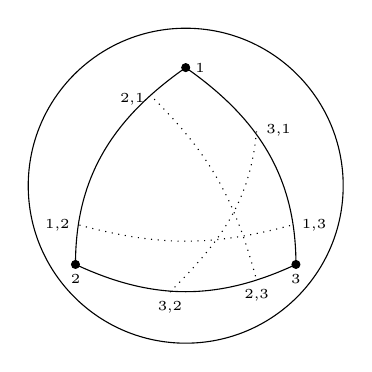
\begin{tikzpicture}
  \draw (2,2) circle [radius=2];

  \draw (0.6, 1) to [out=-25, in=205]
  (3.4, 1) to [out=90, in=-35]
  (2, 3.5) to [out=215, in=90]
  (0.6, 1);
  \draw[fill] (2, 3.5) circle [radius=0.05] node[anchor=west] {\tiny 1};
  \draw[fill] (0.6, 1) circle [radius=0.05] node[anchor=north] {\tiny 2};
  \draw[fill] (3.4, 1) circle [radius=0.05] node[anchor=north] {\tiny 3};
  \draw[dotted] (0.65, 1.5)  node[anchor=east] {\tiny 1,2}
  to [out=-15, in=195] (3.35, 1.5) node[anchor=west] {\tiny 1,3};

  \draw[dotted] (1.8, 0.65) node[anchor=north] {\tiny 3,2}
  to [out=45, in=265] (2.9, 2.7) node[anchor=west] {\tiny 3,1};
  \draw[dotted] (1.6, 3.1) node[anchor=east] {\tiny 2,1}
  to [out=-45, in=105] (2.9, 0.8) node[anchor=north] {\tiny 2,3};
\end{tikzpicture}
\caption{Intersection of great circle arcs inside a spherical triangle,
and the small spherical triangle formed by the arcs. Exaggerated so that the
small triangle is visible; not to scale.}
\label{fig:intlines}
\end{figure}

This method can be extended to the Quadrilateral. Use Slerp to find points on
opposing sides of the quadrilateral, use the cross product to find their
normal, and then use the cross product to find the point of intersection. Since
we draw two intersecting lines, there is only one point of intersection within
the quadrilateral. The formula is:
\begin{equation}\label{eq:gcq}%??? does this reduce to slerp on the edges?
\widetilde{\mathbf v} =
(\mathrm{Slerp}(\mathbf v_1, \mathbf v_2; \frac{u+1}{2})
\times
\mathrm{Slerp}(\mathbf v_4, \mathbf v_3; \frac{u+1}{2}))
\times
(\mathrm{Slerp}(\mathbf v_1, \mathbf v_4; \frac{v+1}{2})
\times
\mathrm{Slerp}(\mathbf v_2, \mathbf v_3; \frac{v+1}{2}))
\end{equation}

This is similar to the Great Circle method, except instead of using the great
circles to calculate the intersections of the lines, we use another spherical
linear interpolation to get a point near the intersection. We effectively use
the Lerp formulas from the section on coordinates, substituting Slerp for Lerp.
Unlike Lerp, Slerp does not commute, so we take the different permutations of
the arguments and combine the different points that result.


(square)
Solve for $u, v$:
\begin{equation}
  \begin{split}
\begin{vmatrix} \mathbf v &
\mathrm{Slerp}(\mathbf v_1, \mathbf v_2; \frac{u+1}{2}) &
\mathrm{Slerp}(\mathbf v_4, \mathbf v_3; \frac{u+1}{2}) \end{vmatrix} &= 0 \\
\begin{vmatrix} \mathbf v &
\mathrm{Slerp}(\mathbf v_1, \mathbf v_4; \frac{v+1}{2}) &
\mathrm{Slerp}(\mathbf v_2, \mathbf v_3; \frac{v+1}{2}) \end{vmatrix} &= 0
\end{split}\end{equation}

\subsection{Naive Slerp}
The Naive Slerp method is derived by a naive analogy with spherical linear
interpolation (Slerp) extended to $uv$ coordinates, thus the
name.

These are two functions that can be derived by analogy with $uv$ coordinates.
Let $w_{ij}$ be the spherical length of the edge between vertices $i$ and $j$.
One:
\begin{equation}\begin{split}\label{eq:nsq1}
   \widetilde{\mathbf v} & = \sum_{i=1}^4\frac{s_i}{\sin(w_u)\sin(w_v)}  \mathbf v_i \\
s_1 & = \sin \left(w_u\frac{1-u}{2}\right)\sin \left(w_v\frac{1-v}{2}\right) \\
s_2 & = \sin \left(w_u\frac{1+u}{2}\right)\sin \left(w_v\frac{1-v}{2}\right) \\
s_3 & = \sin \left(w_u\frac{1+u}{2}\right)\sin \left(w_v\frac{1+v}{2}\right) \\
s_4 & = \sin \left(w_u\frac{1-u}{2}\right)\sin \left(w_v\frac{1+v}{2}\right)
\end{split}\end{equation}
where
\begin{equation}\begin{split}
  w_u &= (1-v) w_{12} + (1+v) w_{34},\\
  w_v &= (1-u) w_{23} + (1+u) w_{14}
\end{split}\end{equation}
Unlike before, the interpolations of $w_u$ and $w_v$ do not have undefined
points. However, they may cause undefined values in the mapping if there is a
point where one is equal to zero.

Two:
\begin{equation}\begin{split}\label{eq:nsq2}
     \widetilde{\mathbf v} & = \sum_{i=1}^4\frac{\sin(w\gamma_i)}{\sin(w)} \mathbf v_i \\
\gamma_1 & = \frac{(1-u)(1-v)}{4} \\
\gamma_2 & = \frac{(1+u)(1-v)}{4} \\
\gamma_3 & = \frac{(1+u)(1+v)}{4} \\
\gamma_4 & = \frac{(1-u)(1+v)}{4}
\end{split}\end{equation}

where
\begin{equation}\begin{split}
  w = \frac{t_{12} w_{12} + t_{23} w_{23} + t_{34} w_{34} + t_{41} w_{41}}
              {t_{12} + t_{23} + t_{34} + t_{41}}\\
  t_{12} &= (1-u)(1-v)(1+u) \\
  t_{23} &= (1-v)(1+u)(1+v) \\
  t_{34} &= (1-u)(1+u)(1+v) \\
  t_{41} &= (1-u)(1-v)(1+v)
\end{split}\end{equation}
Again, this expression is undefined at the vertices, but can be replaced with
any positive value there. If all the edges are equal length, $w$ can be
replaced with that constant edge length.

\subsubsection{Projection of $\widetilde{\mathbf v}$}
The naive slerp methods produces unit vectors along the edges. Because the
projected edges already lie on the sphere, we have freedom in how to adjust
$\widetilde{\mathbf v}$ to lie on the sphere. The easiest is just to centrally
project the vertices, that is, to normalize $\widetilde{\mathbf v}$ like we
have been. Another option is to perform a parallel projection along the
face normal, as defined earlier. We need the parallel distance $p$ from the
vertex to the sphere surface in the direction of the face normal
$\hat{\mathbf n}$, such that $\hat{\mathbf v} =
\widetilde{\mathbf v} + p\hat{\mathbf n}$. $p$ is given by:
\begin{equation}
   p = -\widetilde{\mathbf v} \cdot \hat{\mathbf n} +
   \sqrt{1+\widetilde{\mathbf v} \cdot \hat{\mathbf n}-\widetilde{\mathbf v} \cdot \widetilde{\mathbf v}}
\end{equation}
$p$ can also be approximated as $\widetilde{p} = 1 - \|\widetilde{\mathbf v}\|
\leq p$, which takes fewer operations and doesn't require
calculation of the face normal. Technically, you can project in almost any
direction, not just that of the face normal, but most other choices don't
produce a symmetric result.

Really, the projection can be performed from any point in space. Central
projection uses rays from a point at the center of the sphere, and parallel can
be thought of as using rays from a point at infinity. Instead of specifying the
point, we define a linear combination of the two projections:
\begin{equation}
  \hat{\mathbf v} = \frac{\widetilde{\mathbf v} + kp\mathbf c}{\|\dots\|}
\end{equation}
When $k=0$, that's the central projection: when $k=1$, it's the parallel
projection. $p$ may be replaced by $\widetilde{p}$. If our goal is to optimize
a measurement of the map projection, like conformality or area distortion, we
can do a 1-variable optimization on $k$.

\subsubsection{Spherical rectangle}
Naive slerp 1 simplifies nicely for some particular spherical rectangles and
squares. Let the target rectangle be defined by the points $(-a,-b,c)$,
$(a,-b,c)$, $(a,b,c)$, and $(-a,b,c)$ where $a, b, c$ are in $[0,1]$ and
$a^2 + b^2 + c^2 = 1$. The spherical center of this rectangle, and the face
normal, is $(0,0,1)$. Naive slerp 1 from the standard square to this rectangle
is expressible as so:
\begin{equation}\begin{split}
  \widetilde{x} &= \frac{\sin(\frac{w_u}{2}u) \cos(\frac{w_v}{2}v) }
    {\sqrt{1-b^2}}\\
  \widetilde{y} &= \frac{\cos(\frac{w_u}{2}u) \sin(\frac{w_v}{2}v) }
    {\sqrt{1-a^2}}\\
  \widetilde{z} &=\frac{c}{\sqrt{1-a^2}\sqrt{1-b^2}}
    \cos(\frac{w_u}{2}u) \cos(\frac{w_v}{2}v)
\end{split}\end{equation}
where $cos(w_u) = 1 - 2 a^2$ and $cos(w_v) = 1 - 2 b^2$.

In the case where $a=b$, denote $w = w_u = w_v$,
so the above can be expressed as:
\begin{equation}\begin{split}
  \widetilde{x} &= \frac{\sin\left(\frac{w}{2}(u+v)\right) +
    \sin\left(\frac{w}{2}(u-v)\right)}
    {2\sqrt{1-a^2}}\\
  \widetilde{y} &= \frac{\sin\left(\frac{w}{2}(u+v)\right) -
    \sin\left(\frac{w}{2}(u-v)\right)}
    {2\sqrt{1-a^2}}\\
  \widetilde{z} &=\frac{c}{2-2a^2}\left(\cos\left(\frac{w}{2}(u+v)\right) +
    \cos\left(\frac{w}{2}(u-v)\right)\right)
\end{split}\end{equation}
which demonstrates that this mapping on this polygon preserves diagonal lines.

In the case when $c=0$,
and the spherical rectangle takes up an entire hemisphere, the formula further
reduces to:
\begin{equation}\begin{split}
  \widetilde{x} &= \frac{\sin(\frac{w_x}{2}u) \cos(\frac{w_y}{2}v) }
    {a}\\
  \widetilde{y} &= \frac{\cos(\frac{w_x}{2}u) \sin(\frac{w_y}{2}v) }
    {b}\\
  \widetilde{z} &=0
\end{split}\end{equation}

In the limit where $c=0$ and $b = 0$,
\begin{equation}\begin{split}
  \widetilde{x} &= \sin(\frac{\pi}{2}u) \\
  \widetilde{y} &= v \cos(\frac{\pi}{2}u) \\
  \widetilde{z} &= 0
\end{split}\end{equation}

\subsection{Elliptical}
This quadrilateral map is based on naive slerp 1 on a spherical rectangle, as
described in the previous section. Let the vertices of the rectangle be defined
as before.

$\sin(k x)$ may be approximated as $\sin(k)x$, where the two expressions are
equal at $x=-1,0,1$. Similarly, $\cos(k x)$ may be approximated as
$\sqrt{1 - \sin^2(k) x^2}$. This approximation was applied in \cite{reynolds} to
produce an approximate equal-area homeomorphism, as it maintains the boundary
of the shape where $x=\pm1$ or $y=\pm1$. Applying this approximation
to the equation for naive slerp on a spherical rectangle yields:

\begin{equation}\begin{split}\label{eq:elliptical}
  \widetilde{x} &= au \frac{\sqrt{1-b^2 v^2} }
    {\sqrt{1-b^2}}\\
  \widetilde{y} &= bv \frac{\sqrt{1-a^2 u^2} }
    {\sqrt{1-a^2}}\\
  \widetilde{z} &=c \frac{\sqrt{1-a^2 u^2}\sqrt{1-b^2 v^2} }
    {\sqrt{1-a^2}\sqrt{1-b^2}}
\end{split}\end{equation}

In the case when $c=0$, and the spherical rectangle takes up an entire
hemisphere, the formula reduces to:
\begin{equation}\begin{split}
  \widetilde{x} &= u \sqrt{1-b^2 v^2} \\
  \widetilde{y} &= v \sqrt{1-a^2 u^2} \\
  \widetilde{z} &= 0
\end{split}\end{equation}

When $a=b=\frac{1}{\sqrt{2}}$, this is the Nowell's elliptical function from
the square to the disk.\cite{nowellsq}\cite{fong17} Furthermore, when $c=b=0$,
\begin{equation}\begin{split}
  \widetilde{x} &= u  \\
  \widetilde{y} &= v \sqrt{1 - u^2} \\
  \widetilde{z} &= 0
\end{split}\end{equation}
which is the "squelch" function from the square to the disk in \cite{fong17}.

\subsection{Grid-based}

\subsubsection{Inversion}

\subsubsection{Repeated subdivision}
Method 3 in geodesic dome terms

\section{Analysis}
\subsection{From the sphere to the plane}

\subsection{From the plane to the sphere}

\section{Conclusion}

\bibliographystyle{plain}
\bibliography{references}

\end{document}
